\documentclass{template/openetcs_article}
% Use the option "nocc" if the document is not licensed under Creative Commons
%\documentclass[nocc]{template/openetcs_article}
\usepackage{lipsum,url}
\graphicspath{{./template/}{.}{./images/}}
\begin{document}
\frontmatter
\project{openETCS}

%Please do not change anything above this line
%============================
% The document metadata is defined below

%assign a report number here
\reportnum{OETCS/WP4/D4.2-Draft}

%define your workpackage here
\wp{Work-Package 4: ``Verification and Validation''}

%set a title here
\title{Preliminary safety Evaluation Criteria}

%set a subtitle here
\subtitle{Latex Document Draft}

%set the date of the report here
\date{May 2013\\Revised May 2013}

%define a list of authors and their affiliation here

\author{Jan Welte}

\affiliation{Technische Universität Braunschweig\\
  Institute for Traffic Safety and Automation Engineering \\
  Langer Kamp 8 \\
  38118 Braunschweig\\
  Germany}

% define the coverart
\coverart[width=350pt]{openETCS_EUPL}

%define the type of report
\reporttype{Output for secoundary tool evaluation}


\begin{abstract}
%define an abstract here
  This document presents an overview of the safety related evaluation criteria used within the openETCS document structure and based on this derives evaluation criteria for the choice of suitable tools and methods for all safety activities which have to be performed during the openETCS development process. These criteria are based on the safety activities required in D2.6 and the general concept for an openETCS safety process. 
\end{abstract}

%=============================
%Do not change the next three lines
\maketitle
\tableofcontents
\listoffiguresandtables
\newpage
%=============================

% The actual document starts below this line
%=============================


%Start here

\section{Safety Process}

The EN50128 standard defines safety as the ``freedom from unacceptable levels of risk of harm to people" \cite{EN50128}, which shows that the safety approach required by the CENELEC standards is risk-based. As the risk is defined as the ``combination of the rate of occurrence of accidents and incidents resulting in harm (caused by a hazard) and the degree of severity  of that harm" this approach is based on a probabilistic understanding of event occurrence. The overall relations between all these safety-related terms used to define the safety characteristics and the properties are demonstrated by the Risk-Genesis-Model of Schnieder, which is shown in the following figure \ref{fig:Risiko-Genese-Modell-eng}.

\begin{figure}[h]
\centering
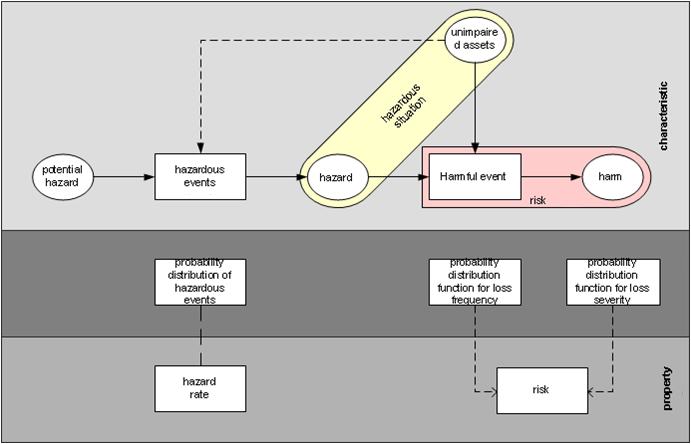
\includegraphics[width=0.7\linewidth]{O:/Projektordner/03_Arbeitsunterlagen/Bearbeitung/WP4/Task4-4/Risiko-Genese-Modell-eng}
\caption{Risk-Genesis-Model showing the relations between the safety-related terms \cite{Schnieder.2010}}
\label{fig:Risiko-Genese-Modell-eng}
\end{figure}

This demonstrates that the first step is to define the system characteristics of a system identifying the harms and their lated hazardous situations. This has to be performed during a system hazard analysis. Afterwards the specific properties of this characteristics have to be defined by assessing the risk concerning the identified hazards. Based on this work safety integrity levels can be determined for all safety functionalities which are then allocated during the design to certain safety-related systems. As this work is closely related to all design decisions, it has to be specified for all abstraction levels during the system design. This leads to safety requirements which have to be implemented in the software design and verified, as well as validated specifically on system level. 

Respectively the EN50126 describes the safety process as a series of safety tasks for each life cycle phase. This task are related to a number of safety artifacts which are created, used and adapted over time by different safety activities.

\subsection{Safety artifacts}

Since all safety activities are based on the system development activities all system design artifacts are part of the safety process. Therefore, the following design artifacts of the CENELEC standard development process build the basis for all safety artifacts:

\begin{itemize}
\item System Concept
\item System Requirements Specification
\item Software Requirement Specification
\item Software Architecture Specification
\item Software Design Specification
\item Software Module Design Specification
\item Software Source Code
\end{itemize}

The main safety artifacts are those which are set-up to build the reference for the safety-related aspect during the system development, which are continuously evolved during the design phases. Correspondingly the safety process has to create artifacts to demonstrated that all safety and quality-related requirements included in the system design. Respectivly the following artifacts are created during the safety process:

\begin{itemize}
\item System Safety Plan
\item Software Quality Assurance Plan
\item Hazard Log
\item System Safety Requirement Specification
\item Safety Case
\end{itemize} 

This artifacts have to be managed over the development process. Since all safety requirement have to be verified and validated there is likewise a close to all Test and Validation Reports.

\subsection{Safety activities}

The safety activities set-up or evolve the safety artifacts in relation to the different design artifacts. Respectively, every activity has certain input and output artifacts as defined in table \ref{tab:SafetyAct}:

\begin{table}[htbp]
\centering
\caption{Safety Activities and their inputs and outputs}
\label{tab:SafetyAct}

\begin{tabular}{|p{5cm}|p{4cm}|p{4cm}|}
\hline \textbf{Safety Activity} & \textbf{Input Artifact(s)} & \textbf{Output Artifact(s)}  \\ 
\hline Preliminary Hazard Analysis & System Concept & Safety Plan \\ 
\hline System Hazard and Safety Risk Analysis & System Concept and Description & Hazard Log \\ 
\hline Risk Assessment & System Concept and Description + Hazard Log & Hazard Log \\ 
\hline Specification of System Safety Requirements & System Requirements Specification + Hazard Log  & System Safety Requirement Specifications \\ 
\hline Define Safety Acceptance Criteria & Hazard Log & Safety Plan  \\ 
\hline Define Safety Related Functional Requirements & System Safety Requirement Specifications & System Requirements Specification  \\ 
\hline Specify Sub-System and Component Safety requirements & System Requirements Specification + System Safety Requirement Specification & System Safety Plan + System Requirements Specification + System Safety Requirement Specification\\
\hline Implement Safety Plan & Safety Plan & Hazard Log + Safety Case \\
\hline Validate System Safety Requirements & System Safety Requirements & Safety Case \\
\hline 
\end{tabular}  
\end{table}

Overall the safety activities have to be performed in close relation to the overall verification and validation activities as these have to verify and validate all safety requirements and their results become part of the safety plan.


\subsection{OpenETCS safety process}

The presented CENELEC standard safety artifacts and activities are always related to the overall system development. Since the openETCS development process just describes the development of the on-board unit software for ETCS additional system informations are needed for the openETCS safety process. These are mainly the following two parts of the CCS TSI:

\begin{itemize}
\item UNISIG SUBSET-026	System Requirements Specification 	(Version 3.3.0)
\item UNISIG SUBSET-091 Safety Requirements for the Technical Interoperability of ETCS in Levels 1 and 2 	(Version 3.2.0)
\end{itemize}

In relation to SUBSET-91 further documents should be considered:

\begin{itemize}
\item Part of TSI Annex A
	\begin{itemize}
	\item SUBSET-036
	\item SUBSET-037
	\item SUBSET-040
	\item SUBSET-041
	\item SUBSET-098
	\end{itemize}
	
\item Not part of TSI Annex A
	\begin{itemize}
	\item SUBSET-039
	\item SUBSET-078
	\item SUBSET-079
	\item SUBSET-080
	\item SUBSET-081
	\item SUBSET-088
	\end{itemize}
\end{itemize}

From these documents the Preliminary Hazard Analysis and the System Safety Goals have to be derived which are needed as the starting point for the openETCS safety process. Based on these information a subsystem hazard and risk analysis for the openETCS scope can be performed which set-up the openETCS hazard log. Based on these results the openETCS safety requirements will be specified, which are then further developed to functional requirements. During the development these requirements are adopted if necessary for the different abstraction levels from the high level model down to the source code. This is done using corresponding safety backlogs, which are the reference for the safety requirement verification. Altogether the source code has to be validated against all safety requirements to demonstrated, that the software can not cause any harm. The safety case has to present all needed documentation.
 
The main task of the openETCS safety process concerning the interactions with the development process are shown in figure \ref{fig:WholeSafetyProcess}.

\begin{figure}[h]
\centering
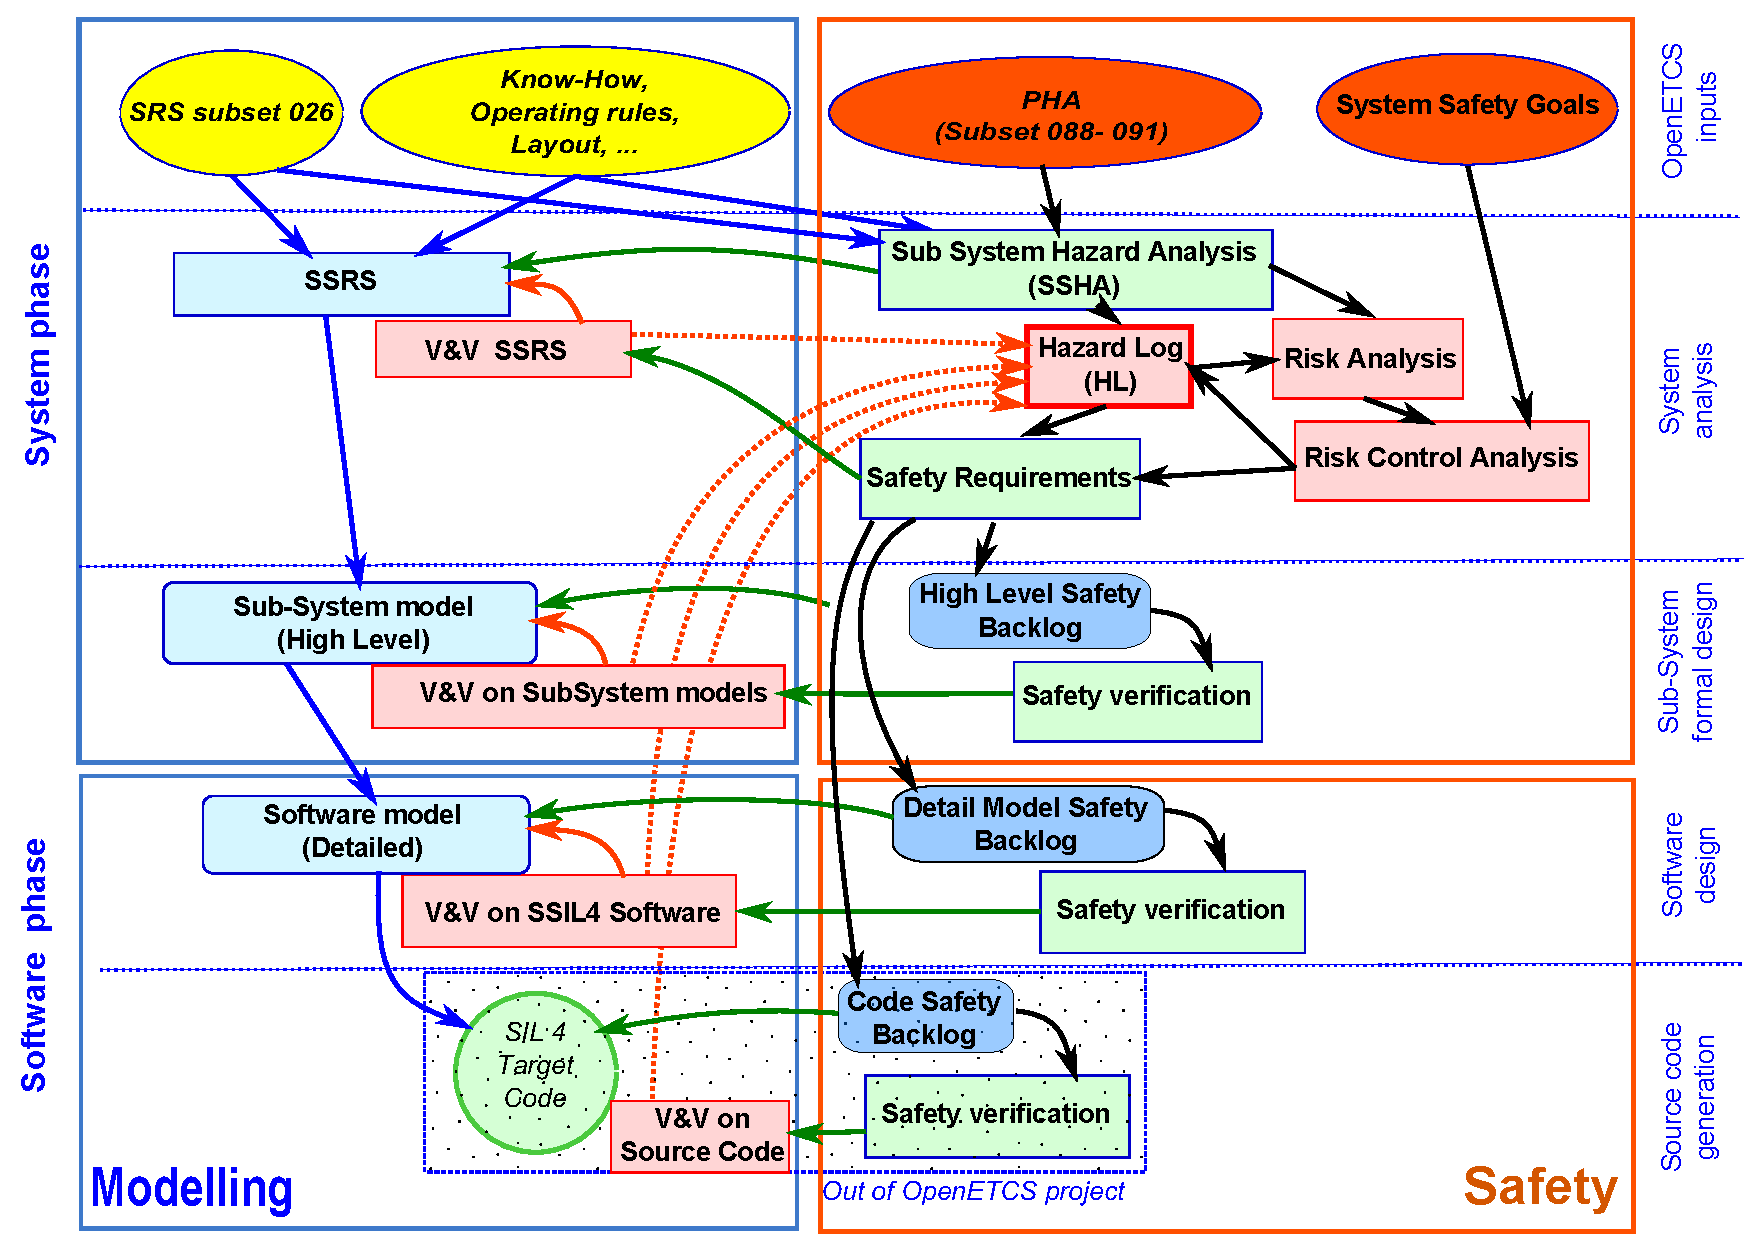
\includegraphics[width=0.8\linewidth]{./images/WholeSafetyProcess}
\caption{OpenETCS Safety Process}
\label{fig:WholeSafetyProcess}
\end{figure}

The openETCS safety process will be specified more detailed in the safety plan. Correspondingly, the main safety artifacts and safety activities which have to be handled during the openETCS safety process are shown in table \ref{tab:openETCS-Safety-artifacts} and \ref{tab:openETCS-Safety-activities}.

% Table generated by Excel2LaTeX from sheet 'Artifact Categorization'
\begin{table}[htbp]
  \centering
  \caption{Main openETCS safety process artifacts}
    \begin{tabular}{r|p{8cm}|p{4cm}}
    \textbf{Abbreviation} & \textbf{Safety Artifact} & \textbf{Degree of Formalisation}\\
    \hline
    Safety Req & Safety Requirements: list of all requirements which have to be respected during the system development to reach the safety goals & Informal/ Semi-Formal / Formal \\
    HL    & Hazard Log: List of identified hazards and its associated risk classification as well as information concerning the risk control & Informal \\
    SP    & Safety Plan: Document which specifies all activities, resources and events to ensure that the source code will satisfy all relevant safety requirements & Informal \\
    SC    & Safety Case: Documentation which demonstrates that the used development process and the resulting source code fulfill all safety requirements & Informal \\
    CSB   & Code Safety Backlog: list of requirements/ properties to be implemented inside the dM derived from  the HL (and the dMSB) & Semi-Formal/ Strictly-Formal \\
    dMSB  & Detailed Model Safety Backlog: list of requirements/ properties to be implemented inside the dM derived from the HL (and  the hLSB) & Semi-Formal/ Strictly-Formal \\
    hLSB  & High Level Safety Backlog: list of requirements/ properties to be implemented inside the hM derived from the HL & Informal/ Semi-Formal \\
    \end{tabular}%
  \label{tab:openETCS-Safety-artifacts}%
\end{table}%

\begin{table}[htbp]
  \centering
  \caption{Main openETCS safety process activities}
    \begin{tabular}{p{6cm}|p{4cm}|p{4cm}} 
 \textbf{Safety Activity} & \textbf{Input Artifact(s)} & \textbf{Output Artifact(s)}  \\ \hline
 Preliminary Hazard Analysis (PHA) & Mainly SUBSET-91 & Safety Plan + Safety Goals \\ 
 Sub-System Hazard and Risk Analysis (SSHA) & Mainly SSRS + Safety Goals & Hazard Log \\ 
 Specification of Sub-System Safety Requirements & SUBSET-26 + SUBSET-91 + Hazard Log  & Safety Requirement Specifications \\ 
 Define Safety Acceptance Criteria & Hazard Log & Safety Plan  \\ 
 Update Hazard Log & Verification Reports + Test Cases & Hazard Log \\
 Specify functional and model specific Requirements & SSRS + Safety Requirement Specification & Safety Plan + Model Backlogs\\
 Verify Safety Requirements & Models + Safety Requirements + Model Backlogs & Verification Report + Safety Case \\
 Validate Safety Requirements & Source Code + Safety Requirements & Validation Report + Safety Case \\
 
\end{tabular}  
  \label{tab:openETCS-Safety-activities}%
\end{table}%

\subsection{Safety process supporting tools}

Supporting software tools are needed to handle the safety artifacts and to some degree to more efficiently perform the safety activities. As some safety artifacts like the safety requirement specifications and the safety backlogs are closely related to design artifacts the same tools can be used. Especially all requirements should be handled by one tool to ensure full traceability and provide one main interface for the verification and validation activities.

Depending on the methods used for hazard and risk analysis appropriate tools are needed to perform the analysis, collect the hazards and associated risks in the hazard log and to evaluated possible risk control measures. Thereby, traceability has to be guarantied between all activities.

Since the safety plan and safety case provide the basis for the safety approval the tools used to generated these artifacts should help to generate a consistent argumentation and efficiently collect the data needed to provide evidence. Respectively, interfaces to manage documents and automatically generate reports would be helpful functionalities.

\section{Evaluation Criteria}

The safety process has to ensure and demonstrated that the development process in general and the specific source code provide adequate protection against all relevant hazards. Therefore the safety process and the supporting tools have to be linked to the development process and especially the requirement handling and verification and validation activities.

\subsection{Safety Process}



\subsection{Supporting tools}


\nocite{*}

\bibliographystyle{unsrt}
\bibliography{erdc}



\begin{thebibliography}{9}



\end{thebibliography}

%===================================================
%Do NOT change anything below this line

\end{document}
